% Options for packages loaded elsewhere
\PassOptionsToPackage{unicode}{hyperref}
\PassOptionsToPackage{hyphens}{url}
%
\documentclass[
  ignorenonframetext,
  t,xcolor=table]{beamer}
\usepackage{pgfpages}
\setbeamertemplate{caption}[numbered]
\setbeamertemplate{caption label separator}{: }
\setbeamercolor{caption name}{fg=normal text.fg}
\beamertemplatenavigationsymbolsempty
% Prevent slide breaks in the middle of a paragraph
\widowpenalties 1 10000
\raggedbottom
\setbeamertemplate{part page}{
  \centering
  \begin{beamercolorbox}[sep=16pt,center]{part title}
    \usebeamerfont{part title}\insertpart\par
  \end{beamercolorbox}
}
\setbeamertemplate{section page}{
  \centering
  \begin{beamercolorbox}[sep=12pt,center]{part title}
    \usebeamerfont{section title}\insertsection\par
  \end{beamercolorbox}
}
\setbeamertemplate{subsection page}{
  \centering
  \begin{beamercolorbox}[sep=8pt,center]{part title}
    \usebeamerfont{subsection title}\insertsubsection\par
  \end{beamercolorbox}
}
\AtBeginPart{
  \frame{\partpage}
}
\AtBeginSection{
  \ifbibliography
  \else
    \frame{\sectionpage}
  \fi
}
\AtBeginSubsection{
  \frame{\subsectionpage}
}
\usepackage{amsmath,amssymb}
\usepackage{iftex}
\ifPDFTeX
  \usepackage[T1]{fontenc}
  \usepackage[utf8]{inputenc}
  \usepackage{textcomp} % provide euro and other symbols
\else % if luatex or xetex
  \usepackage{unicode-math} % this also loads fontspec
  \defaultfontfeatures{Scale=MatchLowercase}
  \defaultfontfeatures[\rmfamily]{Ligatures=TeX,Scale=1}
\fi
\usepackage{lmodern}
\usetheme[]{CambridgeUS}
\usecolortheme{seagull}
\usefonttheme{structurebold}
\ifPDFTeX\else
  % xetex/luatex font selection
\fi
% Use upquote if available, for straight quotes in verbatim environments
\IfFileExists{upquote.sty}{\usepackage{upquote}}{}
\IfFileExists{microtype.sty}{% use microtype if available
  \usepackage[]{microtype}
  \UseMicrotypeSet[protrusion]{basicmath} % disable protrusion for tt fonts
}{}
\makeatletter
\@ifundefined{KOMAClassName}{% if non-KOMA class
  \IfFileExists{parskip.sty}{%
    \usepackage{parskip}
  }{% else
    \setlength{\parindent}{0pt}
    \setlength{\parskip}{6pt plus 2pt minus 1pt}}
}{% if KOMA class
  \KOMAoptions{parskip=half}}
\makeatother
\usepackage{xcolor}
\newif\ifbibliography
\usepackage{color}
\usepackage{fancyvrb}
\newcommand{\VerbBar}{|}
\newcommand{\VERB}{\Verb[commandchars=\\\{\}]}
\DefineVerbatimEnvironment{Highlighting}{Verbatim}{commandchars=\\\{\}}
% Add ',fontsize=\small' for more characters per line
\usepackage{framed}
\definecolor{shadecolor}{RGB}{248,248,248}
\newenvironment{Shaded}{\begin{snugshade}}{\end{snugshade}}
\newcommand{\AlertTok}[1]{\textcolor[rgb]{0.94,0.16,0.16}{#1}}
\newcommand{\AnnotationTok}[1]{\textcolor[rgb]{0.56,0.35,0.01}{\textbf{\textit{#1}}}}
\newcommand{\AttributeTok}[1]{\textcolor[rgb]{0.13,0.29,0.53}{#1}}
\newcommand{\BaseNTok}[1]{\textcolor[rgb]{0.00,0.00,0.81}{#1}}
\newcommand{\BuiltInTok}[1]{#1}
\newcommand{\CharTok}[1]{\textcolor[rgb]{0.31,0.60,0.02}{#1}}
\newcommand{\CommentTok}[1]{\textcolor[rgb]{0.56,0.35,0.01}{\textit{#1}}}
\newcommand{\CommentVarTok}[1]{\textcolor[rgb]{0.56,0.35,0.01}{\textbf{\textit{#1}}}}
\newcommand{\ConstantTok}[1]{\textcolor[rgb]{0.56,0.35,0.01}{#1}}
\newcommand{\ControlFlowTok}[1]{\textcolor[rgb]{0.13,0.29,0.53}{\textbf{#1}}}
\newcommand{\DataTypeTok}[1]{\textcolor[rgb]{0.13,0.29,0.53}{#1}}
\newcommand{\DecValTok}[1]{\textcolor[rgb]{0.00,0.00,0.81}{#1}}
\newcommand{\DocumentationTok}[1]{\textcolor[rgb]{0.56,0.35,0.01}{\textbf{\textit{#1}}}}
\newcommand{\ErrorTok}[1]{\textcolor[rgb]{0.64,0.00,0.00}{\textbf{#1}}}
\newcommand{\ExtensionTok}[1]{#1}
\newcommand{\FloatTok}[1]{\textcolor[rgb]{0.00,0.00,0.81}{#1}}
\newcommand{\FunctionTok}[1]{\textcolor[rgb]{0.13,0.29,0.53}{\textbf{#1}}}
\newcommand{\ImportTok}[1]{#1}
\newcommand{\InformationTok}[1]{\textcolor[rgb]{0.56,0.35,0.01}{\textbf{\textit{#1}}}}
\newcommand{\KeywordTok}[1]{\textcolor[rgb]{0.13,0.29,0.53}{\textbf{#1}}}
\newcommand{\NormalTok}[1]{#1}
\newcommand{\OperatorTok}[1]{\textcolor[rgb]{0.81,0.36,0.00}{\textbf{#1}}}
\newcommand{\OtherTok}[1]{\textcolor[rgb]{0.56,0.35,0.01}{#1}}
\newcommand{\PreprocessorTok}[1]{\textcolor[rgb]{0.56,0.35,0.01}{\textit{#1}}}
\newcommand{\RegionMarkerTok}[1]{#1}
\newcommand{\SpecialCharTok}[1]{\textcolor[rgb]{0.81,0.36,0.00}{\textbf{#1}}}
\newcommand{\SpecialStringTok}[1]{\textcolor[rgb]{0.31,0.60,0.02}{#1}}
\newcommand{\StringTok}[1]{\textcolor[rgb]{0.31,0.60,0.02}{#1}}
\newcommand{\VariableTok}[1]{\textcolor[rgb]{0.00,0.00,0.00}{#1}}
\newcommand{\VerbatimStringTok}[1]{\textcolor[rgb]{0.31,0.60,0.02}{#1}}
\newcommand{\WarningTok}[1]{\textcolor[rgb]{0.56,0.35,0.01}{\textbf{\textit{#1}}}}
\usepackage{graphicx}
\makeatletter
\def\maxwidth{\ifdim\Gin@nat@width>\linewidth\linewidth\else\Gin@nat@width\fi}
\def\maxheight{\ifdim\Gin@nat@height>\textheight\textheight\else\Gin@nat@height\fi}
\makeatother
% Scale images if necessary, so that they will not overflow the page
% margins by default, and it is still possible to overwrite the defaults
% using explicit options in \includegraphics[width, height, ...]{}
\setkeys{Gin}{width=\maxwidth,height=\maxheight,keepaspectratio}
% Set default figure placement to htbp
\makeatletter
\def\fps@figure{htbp}
\makeatother
\setlength{\emergencystretch}{3em} % prevent overfull lines
\providecommand{\tightlist}{%
  \setlength{\itemsep}{0pt}\setlength{\parskip}{0pt}}
\setcounter{secnumdepth}{-\maxdimen} % remove section numbering
%%% Работа с русским языком
\usepackage[russian,english]{babel}   %% загружает пакет многоязыковой вёрстки
% \usepackage{fontspec}      %% подготавливает загрузку шрифтов Open Type, True Type и др.
\defaultfontfeatures{Ligatures={TeX},Renderer=Basic,Scale=0.75}  %% свойства шрифтов по умолчанию
\setmainfont[Ligatures={TeX,Historic}]{Times New Roman} %% задаёт основной шрифт документа
\setsansfont[Ligatures={TeX,Historic}]{Verdana} %% задаёт шрифт без засечек
\setmonofont[Scale=0.7]{DejaVu Sans Mono}

\linespread{0.75}

\definecolor{links}{HTML}{2A1B81}
\hypersetup{colorlinks=true,linkcolor=,urlcolor=links,pdfview=FitH,pdfpagelayout=SinglePage, unicode=true,breaklinks=true}

% % links format
% \usepackage{hyperref}

% decrease text margins
\setbeamersize{text margin left = 8pt, text margin right = 16pt}

% to get bold inside verbatim
\usepackage{listings}
\lstset{basicstyle=\ttfamily,
escapeinside={||},
mathescape=true}


\newcommand{\columnsbegin}{\begin{columns}[T]}
\newcommand{\columnsend}{\end{columns}}
\newcommand{\blockbegin}{\begin{block}}
\newcommand{\blockend}{\end{block}}

% % subfigures
% \usepackage{subcaption}
% \usepackage{wrapfig}

%\addto{\captionsrussian}{\renewcommand*{\figurename}{рис.}}

% Tables
% Define new column types to adjust sizes in tabular environment
% For example, \begin{tabular}{ L{2.3cm} C{2cm} C{1.5cm} C{2.5cm} C{4cm}}
\usepackage{array}
\renewcommand{\arraystretch}{2}
\newcolumntype{L}[1]{>{\raggedright\let\newline\\\arraybackslash\hspace{0pt}}m{#1}}
\newcolumntype{C}[1]{>{\centering\let\newline\\\arraybackslash\hspace{0pt}}m{#1}}
\newcolumntype{R}[1]{>{\raggedleft\let\newline\\\arraybackslash\hspace{0pt}}m{#1}}

% \logo{
\includegraphics[height=0.3cm]{assets/Linmod_logo.png}}


\usepackage{pbox}
\usepackage{bussproofs}

\setbeamertemplate{section page}
{
\vfill
    \begin{centering}
    \begin{beamercolorbox}[sep=12pt,center]{part title}
    \usebeamerfont{section title}\insertsection\par
    \end{beamercolorbox}
    \end{centering}
}
\ifLuaTeX
  \usepackage{selnolig}  % disable illegal ligatures
\fi
\IfFileExists{bookmark.sty}{\usepackage{bookmark}}{\usepackage{hyperref}}
\IfFileExists{xurl.sty}{\usepackage{xurl}}{} % add URL line breaks if available
\urlstyle{same}
\hypersetup{
  pdftitle={Регрессионный анализ, часть 2},
  pdfauthor={Марина Варфоломеева},
  hidelinks,
  pdfcreator={LaTeX via pandoc}}

\title{Регрессионный анализ, часть 2}
\subtitle{Математические методы в зоологии с использованием R}
\author{Марина Варфоломеева}
\date{}

\begin{document}
\frame{\titlepage}

\begin{frame}
\begin{block}{Вы сможете}
\protect\hypertarget{ux432ux44b-ux441ux43cux43eux436ux435ux442ux435}{}
\begin{itemize}
\tightlist
\item
  Подобрать модель множественной линейной регрессии
\item
  Протестировать значимость модели и ее коэффициентов
\item
  Интерпретировать коэффициенты множественной регрессии при разных
  предикторах
\item
  Проверить условия применимости простой и множественной линейной
  регрессии при помощи анализа остатков
\end{itemize}
\end{block}
\end{frame}

\hypertarget{ux43cux43dux43eux436ux435ux441ux442ux432ux435ux43dux43dux430ux44f-ux43bux438ux43dux435ux439ux43dux430ux44f-ux440ux435ux433ux440ux435ux441ux441ux438ux44f}{%
\section{Множественная линейная
регрессия}\label{ux43cux43dux43eux436ux435ux441ux442ux432ux435ux43dux43dux430ux44f-ux43bux438ux43dux435ux439ux43dux430ux44f-ux440ux435ux433ux440ux435ux441ux441ux438ux44f}}

\begin{frame}[fragile]{Пример: птицы Австралии}
\protect\hypertarget{ux43fux440ux438ux43cux435ux440-ux43fux442ux438ux446ux44b-ux430ux432ux441ux442ux440ux430ux43bux438ux438}{}
Зависит ли обилие птиц в лесах Австралии от характеристик леса? (Loyn,
1987, пример из кн. Quinn, Keough, 2002)

56 лесных участков в юго-восточной Виктории, Австралия

\begin{itemize}
\tightlist
\item
  \texttt{l10area} - Площадь леса, га (логарифм)
\item
  \texttt{l10dist} - Расстояние до ближайшего леса, км (логарифм)
\item
  \texttt{l10ldist} - Расстояние до ближайшего леса большего размера, км
  (логарифм)
\item
  \texttt{yr.isol} - Год начала изоляции
\item
  \texttt{abund} - Обилие птиц
\end{itemize}
\end{frame}

\begin{frame}[fragile]{Читаем данные из файла одним из способов}
\protect\hypertarget{ux447ux438ux442ux430ux435ux43c-ux434ux430ux43dux43dux44bux435-ux438ux437-ux444ux430ux439ux43bux430-ux43eux434ux43dux438ux43c-ux438ux437-ux441ux43fux43eux441ux43eux431ux43eux432}{}
\begin{block}{Чтение из xlsx}
\protect\hypertarget{ux447ux442ux435ux43dux438ux435-ux438ux437-xlsx}{}
\begin{Shaded}
\begin{Highlighting}[]
\FunctionTok{library}\NormalTok{(readxl)}
\NormalTok{bird }\OtherTok{\textless{}{-}} \FunctionTok{read\_excel}\NormalTok{(}\AttributeTok{path =} \StringTok{"data/loyn.xlsx"}\NormalTok{, }\AttributeTok{sheet =} \DecValTok{1}\NormalTok{)}
\end{Highlighting}
\end{Shaded}
\end{block}

\begin{block}{Чтение из csv}
\protect\hypertarget{ux447ux442ux435ux43dux438ux435-ux438ux437-csv}{}
\begin{Shaded}
\begin{Highlighting}[]
\NormalTok{bird }\OtherTok{\textless{}{-}} \FunctionTok{read.table}\NormalTok{(}\StringTok{"data/loyn.csv"}\NormalTok{, }\AttributeTok{header =} \ConstantTok{TRUE}\NormalTok{, }\AttributeTok{sep =} \StringTok{"}\SpecialCharTok{\textbackslash{}t}\StringTok{"}\NormalTok{)}
\end{Highlighting}
\end{Shaded}
\end{block}
\end{frame}

\begin{frame}[fragile]{Все ли правильно открылось?}
\protect\hypertarget{ux432ux441ux435-ux43bux438-ux43fux440ux430ux432ux438ux43bux44cux43dux43e-ux43eux442ux43aux440ux44bux43bux43eux441ux44c}{}
\begin{Shaded}
\begin{Highlighting}[]
\FunctionTok{str}\NormalTok{(bird)      }\CommentTok{\# Структура данных}
\end{Highlighting}
\end{Shaded}

\begin{verbatim}
# 'data.frame': 56 obs. of  10 variables:
#  $ abund   : num  5.3 2 1.5 17.1 13.8 14.1 3.8 2.2 3.3 3 ...
#  $ area    : num  0.1 0.5 0.5 1 1 1 1 1 1 1 ...
#  $ yr.isol : int  1968 1920 1900 1966 1918 1965 1955 1920 1965 1900 ...
#  $ dist    : int  39 234 104 66 246 234 467 284 156 311 ...
#  $ ldist   : int  39 234 311 66 246 285 467 1829 156 571 ...
#  $ graze   : int  2 5 5 3 5 3 5 5 4 5 ...
#  $ alt     : int  160 60 140 160 140 130 90 60 130 130 ...
#  $ l10dist : num  1.59 2.37 2.02 1.82 2.39 ...
#  $ l10ldist: num  1.59 2.37 2.49 1.82 2.39 ...
#  $ l10area : num  -1 -0.301 -0.301 0 0 ...
\end{verbatim}

\begin{Shaded}
\begin{Highlighting}[]
\FunctionTok{head}\NormalTok{(bird)     }\CommentTok{\# Первые несколько строк файла}
\end{Highlighting}
\end{Shaded}

\begin{verbatim}
#   abund area yr.isol dist ldist graze alt l10dist l10ldist l10area
# 1   5.3  0.1    1968   39    39     2 160   1.591    1.591  -1.000
# 2   2.0  0.5    1920  234   234     5  60   2.369    2.369  -0.301
# 3   1.5  0.5    1900  104   311     5 140   2.017    2.493  -0.301
# 4  17.1  1.0    1966   66    66     3 160   1.820    1.820   0.000
# 5  13.8  1.0    1918  246   246     5 140   2.391    2.391   0.000
# 6  14.1  1.0    1965  234   285     3 130   2.369    2.455   0.000
\end{verbatim}
\end{frame}

\begin{frame}[fragile]{Знакомимся с данными}
\protect\hypertarget{ux437ux43dux430ux43aux43eux43cux438ux43cux441ux44f-ux441-ux434ux430ux43dux43dux44bux43cux438}{}
Есть ли пропущенные значения?

\begin{Shaded}
\begin{Highlighting}[]
\FunctionTok{colSums}\NormalTok{(}\FunctionTok{is.na}\NormalTok{(bird))}
\end{Highlighting}
\end{Shaded}

\begin{verbatim}
#    abund     area  yr.isol     dist    ldist    graze      alt 
#        0        0        0        0        0        0        0 
#  l10dist l10ldist  l10area 
#        0        0        0
\end{verbatim}

Каков объем выборки?

\begin{Shaded}
\begin{Highlighting}[]
\FunctionTok{nrow}\NormalTok{(bird)}
\end{Highlighting}
\end{Shaded}

\begin{verbatim}
# [1] 56
\end{verbatim}
\end{frame}

\begin{frame}[fragile]{Задача}
\protect\hypertarget{ux437ux430ux434ux430ux447ux430}{}
\begin{enumerate}
\tightlist
\item
  Подберите модель множественной линейной регрессии, чтобы описать, как
  зависит обилие птиц от характеристик леса
\item
  Проверьте значимость ее коэффициентов при помощи t-критерия
\end{enumerate}

\vfill

Предикторы:

\begin{itemize}
\tightlist
\item
  \texttt{abund} - Обилие птиц
\item
  \texttt{l10area} - Площадь леса, га
\item
  \texttt{l10dist} - Расстояние до ближайшего леса, км (логарифм)
\item
  \texttt{l10ldist} - Расстояние до ближайшего леса большего размера, км
  (логарифм)
\item
  \texttt{yr.isol} - Год изоляции лесного массива
\end{itemize}
\end{frame}

\begin{frame}[fragile]{Решение}
\protect\hypertarget{ux440ux435ux448ux435ux43dux438ux435}{}
\fontsize{10pt}{10pt}

\begin{Shaded}
\begin{Highlighting}[]
\NormalTok{bird\_lm }\OtherTok{\textless{}{-}} \FunctionTok{lm}\NormalTok{(abund }\SpecialCharTok{\textasciitilde{}}\NormalTok{ l10area }\SpecialCharTok{+}\NormalTok{ l10dist }\SpecialCharTok{+}\NormalTok{ l10ldist }\SpecialCharTok{+}\NormalTok{ yr.isol, }\AttributeTok{data =}\NormalTok{ bird)}
\FunctionTok{summary}\NormalTok{(bird\_lm)}
\end{Highlighting}
\end{Shaded}

\begin{verbatim}
# 
# Call:
# lm(formula = abund ~ l10area + l10dist + l10ldist + yr.isol, 
#     data = bird)
# 
# Residuals:
#     Min      1Q  Median      3Q     Max 
# -16.663  -3.546   0.086   2.884  16.530 
# 
# Coefficients:
#              Estimate Std. Error t value     Pr(>|t|)    
# (Intercept) -224.4246    74.8504   -3.00       0.0042 ** 
# l10area        9.2348     1.2760    7.24 0.0000000023 ***
# l10dist       -0.7046     2.7077   -0.26       0.7957    
# l10ldist      -1.5935     2.0954   -0.76       0.4505    
# yr.isol        0.1236     0.0379    3.26       0.0020 ** 
# ---
# Signif. codes:  0 '***' 0.001 '**' 0.01 '*' 0.05 '.' 0.1 ' ' 1
# 
# Residual standard error: 6.58 on 51 degrees of freedom
# Multiple R-squared:  0.652,   Adjusted R-squared:  0.625 
# F-statistic: 23.9 on 4 and 51 DF,  p-value: 3.62e-11
\end{verbatim}
\end{frame}

\begin{frame}{Можно привести результаты t-теста для коэффициентов в виде
таблицы}
\protect\hypertarget{ux43cux43eux436ux43dux43e-ux43fux440ux438ux432ux435ux441ux442ux438-ux440ux435ux437ux443ux43bux44cux442ux430ux442ux44b-t-ux442ux435ux441ux442ux430-ux434ux43bux44f-ux43aux43eux44dux444ux444ux438ux446ux438ux435ux43dux442ux43eux432-ux432-ux432ux438ux434ux435-ux442ux430ux431ux43bux438ux446ux44b}{}
Обилие птиц увеличивалось с увеличением площади леса, и с уменьшением
продолжительности изоляции (Табл. \autoref{tab:mreg-coef}).

\begin{table}[ht]
\centering
\caption{Коэффициенты линейной регрессии обилия птиц от различных характеристик леса: l10area - логарифм площади леса, l10dist --- логарифм расстояния до ближайшего леса, l10ldist --- логарифм расстояния до ближайшего большого леса, yr.isol --- год изоляции лесного массива. t --- значение t-критерия, P --- уровень значимости.} 
\label{tab:mreg-coef}
\begin{tabular}{rrrrl}
  \hline
 & Оценка & Ст.ошибка & t & P \\ 
  \hline
Отрезок & -224.42 & 74.85 & -3.00 & $<$0.01 \\ 
  l10area & 9.23 & 1.28 & 7.24 & $<$0.01 \\ 
  l10dist & -0.70 & 2.71 & -0.26 & 0.80 \\ 
  l10ldist & -1.59 & 2.10 & -0.76 & 0.45 \\ 
  yr.isol & 0.12 & 0.04 & 3.26 & $<$0.01 \\ 
   \hline
\end{tabular}
\end{table}

Можно было бы нарисовать график предсказаний модели, но в этом курсе мы
не будем это разбирать
\end{frame}

\begin{frame}{Задача}
\protect\hypertarget{ux437ux430ux434ux430ux447ux430-1}{}
Запишите уравнение множественной линейной регрессии
\end{frame}

\begin{frame}[fragile]{Решение}
\protect\hypertarget{ux440ux435ux448ux435ux43dux438ux435-1}{}
Коэффициенты модели:

\begin{Shaded}
\begin{Highlighting}[]
\FunctionTok{coef}\NormalTok{(bird\_lm)}
\end{Highlighting}
\end{Shaded}

\begin{verbatim}
# (Intercept)     l10area     l10dist    l10ldist     yr.isol 
#   -224.4246      9.2348     -0.7046     -1.5935      0.1236
\end{verbatim}

Уравнение регрессии:

\(abund _i = - 224.42 + 9.23 l10area _i - 0.70 l10dist _i - 1.59 l10ldist _i + 0.12 yr.isol_i\)

Более формальная запись:

\(Y_i = - 224.42 + 9.23 X_{1i} - 0.70 X_{2i} - 1.59 X_{3i} + 0.12 X_{4i}\)
\end{frame}

\begin{frame}[fragile]{Интерпретация коэффициентов регрессии}
\protect\hypertarget{ux438ux43dux442ux435ux440ux43fux440ux435ux442ux430ux446ux438ux44f-ux43aux43eux44dux444ux444ux438ux446ux438ux435ux43dux442ux43eux432-ux440ux435ux433ux440ux435ux441ux441ux438ux438}{}
\begin{Shaded}
\begin{Highlighting}[]
\FunctionTok{coef}\NormalTok{(bird\_lm)}
\end{Highlighting}
\end{Shaded}

\begin{verbatim}
# (Intercept)     l10area     l10dist    l10ldist     yr.isol 
#   -224.4246      9.2348     -0.7046     -1.5935      0.1236
\end{verbatim}

\pause

\begin{block}{Обычные коэффициенты}
\protect\hypertarget{ux43eux431ux44bux447ux43dux44bux435-ux43aux43eux44dux444ux444ux438ux446ux438ux435ux43dux442ux44b}{}
\begin{itemize}
\tightlist
\item
  Величина обычных коэффициентов зависит от единиц измерения
\item
  \(b_0\) --- Отрезок (Intercept), отсекаемый регрессионной прямой на
  оси \(y\). Значение зависимой переменной \(Y\), если предикторы равны
  нулю.
\item
  Коэффициенты при предикторах показывают, на сколько изменяется \(Y\),
  когда данный предиктор меняется на единицу, при условии, что остальные
  предикторы не меняют своих значений.
\end{itemize}
\end{block}
\end{frame}

\begin{frame}[fragile]{Для сравнения влияния разных предикторов ---
стандартизованные коэффициенты}
\protect\hypertarget{ux434ux43bux44f-ux441ux440ux430ux432ux43dux435ux43dux438ux44f-ux432ux43bux438ux44fux43dux438ux44f-ux440ux430ux437ux43dux44bux445-ux43fux440ux435ux434ux438ux43aux442ux43eux440ux43eux432-ux441ux442ux430ux43dux434ux430ux440ux442ux438ux437ux43eux432ux430ux43dux43dux44bux435-ux43aux43eux44dux444ux444ux438ux446ux438ux435ux43dux442ux44b}{}
\fontsize{10pt}{10pt}

\begin{Shaded}
\begin{Highlighting}[]
\NormalTok{scaled\_bird\_lm }\OtherTok{\textless{}{-}} \FunctionTok{lm}\NormalTok{(abund }\SpecialCharTok{\textasciitilde{}} \FunctionTok{scale}\NormalTok{(l10area) }\SpecialCharTok{+} \FunctionTok{scale}\NormalTok{(l10dist) }\SpecialCharTok{+} 
                       \FunctionTok{scale}\NormalTok{(l10ldist) }\SpecialCharTok{+} \FunctionTok{scale}\NormalTok{(yr.isol), }\AttributeTok{data =}\NormalTok{ bird)}
\FunctionTok{coef}\NormalTok{(scaled\_bird\_lm)}
\end{Highlighting}
\end{Shaded}

\begin{verbatim}
#     (Intercept)  scale(l10area)  scale(l10dist) scale(l10ldist) 
#         19.5143          7.5024         -0.2916         -0.9161 
#  scale(yr.isol) 
#          3.1613
\end{verbatim}

\pause

\begin{block}{Стандартизованные коэффициенты}
\protect\hypertarget{ux441ux442ux430ux43dux434ux430ux440ux442ux438ux437ux43eux432ux430ux43dux43dux44bux435-ux43aux43eux44dux444ux444ux438ux446ux438ux435ux43dux442ux44b}{}
\begin{itemize}
\tightlist
\item
  Стандартизованные коэффициенты измерены в стандартных отклонениях. Их
  можно сравнивать друг с другом, поскольку они дают относительную
  оценку влияния фактора.
\item
  \(b_0\) --- Отрезок (Intercept), отсекаемый регрессионной прямой на
  оси \(y\). Значение зависимой переменной \(Y\), если предикторы равны
  нулю. Для стандартизованных величин среднее значение равно нулю,
  поэтому \(b_0\) --- это значение зависимой переменной при средних
  значениях всех предикторов.
\item
  Коэффициенты при предикторах показывают, на сколько изменяется \(Y\),
  когда предиктор меняется на одно стандартное отклонение, при условии,
  что остальные предикторы не меняют своих значений. Это относительная
  оценка влияния фактора.
\end{itemize}
\end{block}
\end{frame}

\begin{frame}[fragile]{Задача}
\protect\hypertarget{ux437ux430ux434ux430ux447ux430-2}{}
Определите по значениям стандартизованных коэффициентов, какие
предикторы сильнее всего влияют на обилие птиц

\fontsize{10pt}{10pt}

\begin{Shaded}
\begin{Highlighting}[]
\FunctionTok{summary}\NormalTok{(scaled\_bird\_lm)}
\end{Highlighting}
\end{Shaded}

\begin{verbatim}
# 
# Call:
# lm(formula = abund ~ scale(l10area) + scale(l10dist) + scale(l10ldist) + 
#     scale(yr.isol), data = bird)
# 
# Residuals:
#     Min      1Q  Median      3Q     Max 
# -16.663  -3.546   0.086   2.884  16.530 
# 
# Coefficients:
#                 Estimate Std. Error t value     Pr(>|t|)    
# (Intercept)       19.514      0.879   22.20      < 2e-16 ***
# scale(l10area)     7.502      1.037    7.24 0.0000000023 ***
# scale(l10dist)    -0.292      1.120   -0.26        0.796    
# scale(l10ldist)   -0.916      1.205   -0.76        0.450    
# scale(yr.isol)     3.161      0.971    3.26        0.002 ** 
# ---
# Signif. codes:  0 '***' 0.001 '**' 0.01 '*' 0.05 '.' 0.1 ' ' 1
# 
# Residual standard error: 6.58 on 51 degrees of freedom
# Multiple R-squared:  0.652,   Adjusted R-squared:  0.625 
# F-statistic: 23.9 on 4 and 51 DF,  p-value: 3.62e-11
\end{verbatim}
\end{frame}

\begin{frame}[fragile]{Оценка качества подгонки модели}
\protect\hypertarget{ux43eux446ux435ux43dux43aux430-ux43aux430ux447ux435ux441ux442ux432ux430-ux43fux43eux434ux433ux43eux43dux43aux438-ux43cux43eux434ux435ux43bux438}{}
\begin{Shaded}
\begin{Highlighting}[]
\FunctionTok{summary}\NormalTok{(bird\_lm)}\SpecialCharTok{$}\NormalTok{adj.r.squared}
\end{Highlighting}
\end{Shaded}

\begin{verbatim}
# [1] 0.6246
\end{verbatim}

\begin{block}{Обычный \(R^2\) --- доля объясненной изменчивости}
\protect\hypertarget{ux43eux431ux44bux447ux43dux44bux439-r2-ux434ux43eux43bux44f-ux43eux431ux44aux44fux441ux43dux435ux43dux43dux43eux439-ux438ux437ux43cux435ux43dux447ux438ux432ux43eux441ux442ux438}{}
\[R^2 =\frac{SS_{r}}{SS_{t}} = 1 - \frac{SS_{e}}{SS_{t}}\]

\textbf{Не используйте обычный \(R^2\) для множественной регрессии!}
\end{block}

\begin{block}{\(R^2_{adj}\) --- cкорректированный \(R^2\)}
\protect\hypertarget{r2_adj-cux43aux43eux440ux440ux435ux43aux442ux438ux440ux43eux432ux430ux43dux43dux44bux439-r2}{}
\[R^2_{adj} = 1 - (1 - R^2) \frac{n - 1}{n - p}\]

где \(n - p = df_{e}\), \(n - 1 = df_{t}\)

\(R^2_{adj}\) учитывает число переменных в модели, вводится штраф за
каждый новый параметр.

Используйте \(R^2 _{adj}\) для сравнения моделей с разным числом
параметров.
\end{block}
\end{frame}

\hypertarget{ux443ux441ux43bux43eux432ux438ux44f-ux43fux440ux438ux43cux435ux43dux438ux43cux43eux441ux442ux438-ux43bux438ux43dux435ux439ux43dux43eux439-ux440ux435ux433ux440ux435ux441ux441ux438ux438}{%
\section{Условия применимости линейной
регрессии}\label{ux443ux441ux43bux43eux432ux438ux44f-ux43fux440ux438ux43cux435ux43dux438ux43cux43eux441ux442ux438-ux43bux438ux43dux435ux439ux43dux43eux439-ux440ux435ux433ux440ux435ux441ux441ux438ux438}}

\begin{frame}{Условия применимости линейной регрессии}
\protect\hypertarget{ux443ux441ux43bux43eux432ux438ux44f-ux43fux440ux438ux43cux435ux43dux438ux43cux43eux441ux442ux438-ux43bux438ux43dux435ux439ux43dux43eux439-ux440ux435ux433ux440ux435ux441ux441ux438ux438-1}{}
Условия применимости линейной регрессии должны выполняться, чтобы
тестировать гипотезы

\begin{enumerate}
\tightlist
\item
  Независимость
\item
  Линейность
\item
  Нормальное распределение
\item
  Гомогенность дисперсий
\item
  Отсутствие коллинеарности предикторов (для множественной регрессии)
\end{enumerate}
\end{frame}

\begin{frame}{1. Независимость}
\protect\hypertarget{ux43dux435ux437ux430ux432ux438ux441ux438ux43cux43eux441ux442ux44c}{}
\begin{itemize}
\tightlist
\item
  Значения \(y _i\) должны быть независимы друг от друга
\item
  Берегитесь псевдоповторностей и автокорреляций (например, временных)
\item
  Контролируется на этапе планирования
\item
  Проверяем на графике остатков
\end{itemize}

\vskip0pt plus 1filll \centering
\includegraphics[width=0.85\linewidth,keepaspectratio]{images/assumption-12.png}

\raggedright

\tiny Из кн. Diez et al., 2010, стр. 332, рис. 7.8
\end{frame}

\begin{frame}{2. Линейность связи}
\protect\hypertarget{ux43bux438ux43dux435ux439ux43dux43eux441ux442ux44c-ux441ux432ux44fux437ux438}{}
\begin{itemize}
\tightlist
\item
  Проверяем на графике рассеяния исходных данных
\item
  Проверяем на графике остатков
\end{itemize}

\vskip0pt plus 1filll \centering
\includegraphics[width=0.85\linewidth,keepaspectratio]{images/assumption-12.png}

\raggedright

\tiny Из кн. Diez et al., 2010, стр. 332, рис. 7.8
\end{frame}

\begin{frame}{Что бывает, если не глядя применять линейную регрессию}
\protect\hypertarget{ux447ux442ux43e-ux431ux44bux432ux430ux435ux442-ux435ux441ux43bux438-ux43dux435-ux433ux43bux44fux434ux44f-ux43fux440ux438ux43cux435ux43dux44fux442ux44c-ux43bux438ux43dux435ux439ux43dux443ux44e-ux440ux435ux433ux440ux435ux441ux441ux438ux44e}{}
\columnsbegin
\column{0.48\textwidth}

\href{http://ru.wikipedia.org/wiki/Квартет_Энскомба}{Квартет Энскомба} -
примеры данных, где регрессии одинаковы во всех случаях (Anscombe, 1973)

\[y _i = 3.0 + 0.5 x _i\]

\[r^2 = 0.68\]

\[H _0: \beta _1 = 0, t = 4.24, p = 0.002\]

\column{0.48\textwidth}

\centering

\includegraphics[width=\linewidth,height=\textheight,keepaspectratio]{images/anscombe.png}

\raggedright

\tiny Из кн. Quinn, Keough, 2002, стр. 97, рис. 5.9

\columnsend
\end{frame}

\begin{frame}{3. Нормальное распределение остатков}
\protect\hypertarget{ux43dux43eux440ux43cux430ux43bux44cux43dux43eux435-ux440ux430ux441ux43fux440ux435ux434ux435ux43bux435ux43dux438ux435-ux43eux441ux442ux430ux442ux43aux43eux432}{}
\columnsbegin
\column{0.48\textwidth}

Нужно, т.к. в модели \(Y _i = \beta _0 + \beta x _i + \epsilon _i\)
зависимая переменная \(Y \sim N(0,\sigma^2)\), а значит
\(\epsilon _i \sim N(0,\sigma^2)\)

\begin{itemize}
\tightlist
\item
  Нужно для тестов параметров, а не для подбора методом наименьших
  квадратов
\item
  Нарушение не страшно --- тесты устойчивы к небольшим отклонениям от
  нормального распределения
\item
  Проверяем распределение остатков на нормально-вероятностном графике
\end{itemize}

\column{0.48\textwidth}

\centering

\includegraphics[width=\linewidth,height=\textheight,keepaspectratio]{images/normality-assumption.png}

\raggedright

\tiny Из кн. Watkins et al., 2008, стр. 743, рис. 11.4

\columnsend
\end{frame}

\begin{frame}{4. Гомогенность дисперсий}
\protect\hypertarget{ux433ux43eux43cux43eux433ux435ux43dux43dux43eux441ux442ux44c-ux434ux438ux441ux43fux435ux440ux441ux438ux439}{}
\columnsbegin
\column{0.48\textwidth}

Нужно, т.к. в модели \(Y _i = \beta _0 + \beta x _i + \epsilon _i\)
зависимая переменная \(Y \sim N(0,\sigma^2)\) и дисперсии
\(\sigma^2 _1 = \sigma^2 _2 = ... = \sigma^2 _i\) для каждого \(Y _i\)

\par

Но, поскольку \(\epsilon _i \sim N(0,\sigma^2)\), можно проверить
равенство дисперсий остатков \(\epsilon _i\)

\begin{itemize}
\tightlist
\item
  Нужно и важно для тестов параметров
\item
  Проверяем на графике остатков по отношению к предсказанным значениям
\item
  Есть формальные тесты, но они очень чувствительны (тест Бройша-Пагана,
  тест Кокрана)
\end{itemize}

\column{0.48\textwidth}

\centering

\includegraphics[width=\linewidth,height=\textheight,keepaspectratio]{images/normality-assumption.png}

\raggedright

\tiny Из кн. Watkins et al., 2008, стр. 743, рис. 11.4

\columnsend
\end{frame}

\begin{frame}{Диагностика регрессии по графикам остатков}
\protect\hypertarget{ux434ux438ux430ux433ux43dux43eux441ux442ux438ux43aux430-ux440ux435ux433ux440ux435ux441ux441ux438ux438-ux43fux43e-ux433ux440ux430ux444ux438ux43aux430ux43c-ux43eux441ux442ux430ux442ux43aux43eux432}{}
\columnsbegin
\column{0.48\textwidth}

\centering

\includegraphics[width=\linewidth,height=\textheight,keepaspectratio]{images/assumption-violations-on-residual-plots.png}

\raggedright

\tiny Из кн. Logan, 2010, стр. 174, рис. 8.5 d

\column{0.48\textwidth}

\begin{itemize}
\tightlist
\item
  (a)все условия выполнены\\
\item
  (b)разброс остатков разный (wedge-shaped pattern)\\
\item
  (c)разброс остатков одинаковый, но нужны дополнительные предикторы\\
\item
  (d)к нелинейной зависимости применили линейную регрессию
\end{itemize}

\columnsend
\end{frame}

\begin{frame}{Задача: Проанализируйте графики остатков}
\protect\hypertarget{ux437ux430ux434ux430ux447ux430-ux43fux440ux43eux430ux43dux430ux43bux438ux437ux438ux440ux443ux439ux442ux435-ux433ux440ux430ux444ux438ux43aux438-ux43eux441ux442ux430ux442ux43aux43eux432}{}
Скажите пожалуйста

\begin{itemize}
\tightlist
\item
  какой регрессии соответствует какой график остатков?
\item
  все ли условия применимости регрессии здесь выполняются?
\item
  назовите случаи, в которых можно и нельзя применить линейную
  регрессию?
\end{itemize}

\columnsbegin
\column{0.48\textwidth}

\centering

\includegraphics[width=\linewidth,height=\textheight,keepaspectratio]{images/assumption-quiz1.png}

\column{0.48\textwidth}

\includegraphics[width=\linewidth,height=\textheight,keepaspectratio]{images/assumption-quiz2.png}

\columnsend

\tiny\{Из кн. Watkins et al.~2008, стр. 177, рис. 3.84-3.85\}
\end{frame}

\begin{frame}{Решение}
\protect\hypertarget{ux440ux435ux448ux435ux43dux438ux435-2}{}
\begin{itemize}
\tightlist
\item
  A-I - нелинейная связь - нельзя;
\item
  B-II - все в порядке, можно;
\item
  C-III - все в порядке, можно;
\item
  D-IV - синусоидальный паттерн в остатках, нарушено условие
  независимости или зависимость нелинейная - нельзя.
\end{itemize}

\vskip0pt plus 1filll

\columnsbegin
\column{0.48\textwidth}
\centering

\includegraphics[width=\linewidth,height=\textheight,keepaspectratio]{images/assumption-quiz1.png}
\column{0.48\textwidth}

\includegraphics[width=\linewidth,height=\textheight,keepaspectratio]{images/assumption-quiz2.png}
\columnsend

\tiny Рис. из кн. Watkins et al.~2008, стр. 177, рис. 3.84-3.85
\end{frame}

\begin{frame}{Какие наблюдения влияют на ход регрессии больше других?}
\protect\hypertarget{ux43aux430ux43aux438ux435-ux43dux430ux431ux43bux44eux434ux435ux43dux438ux44f-ux432ux43bux438ux44fux44eux442-ux43dux430-ux445ux43eux434-ux440ux435ux433ux440ux435ux441ux441ux438ux438-ux431ux43eux43bux44cux448ux435-ux434ux440ux443ux433ux438ux445}{}
\columnsbegin
\column{0.48\textwidth}

Влиятельные наблюдения, выбросы, outliers

\begin{itemize}
\tightlist
\item
  большая абсолютная величина остатка
\item
  близость к краям области определения (leverage - рычаг, сила; иногда
  называют hat)
\end{itemize}

На графике точки и линии регрессии построенные с их включением:

\begin{itemize}
\tightlist
\item
  1 - не влияет на ход регрессии, т.к. лежит на прямой
\item
  2 - умеренно влияет (большой остаток, малая сила влияния)
\item
  3 - очень сильно влияет (большой остаток, большая сила влияния)
\end{itemize}

\column{0.48\textwidth}

\centering

\includegraphics[width=\linewidth,height=\textheight,keepaspectratio]{images/influential-observations.png}

\raggedright

\tiny Из кн. Quinn, Keough, 2002, стр. 96, рис. 5.8

\columnsend
\end{frame}

\begin{frame}{Как оценить влиятельность наблюдений?}
\protect\hypertarget{ux43aux430ux43a-ux43eux446ux435ux43dux438ux442ux44c-ux432ux43bux438ux44fux442ux435ux43bux44cux43dux43eux441ux442ux44c-ux43dux430ux431ux43bux44eux434ux435ux43dux438ux439}{}
\columnsbegin
\column{0.48\textwidth}

\blockbegin{Расстояние Кука (Cook's d, Cook, 1977)}

\begin{itemize}
\tightlist
\item
  Учитывает одновременно величину остатка и близость к краям области
  определения (leverage)
\item
  Условное пороговое значение: выброс, если \(d \ge 4/(n - p)\), где
  \(n\) - объем выборки, \(p\) - число параметров модели.
\end{itemize}

\blockend

\column{0.48\textwidth}

\centering

\includegraphics[width=\linewidth,height=\textheight,keepaspectratio]{images/influential-observations.png}

\raggedright

\tiny Из кн. Quinn, Keough, 2002, стр. 96, рис. 5.8

\columnsend

\pause

\begin{itemize}
\tightlist
\item
  Дж. Фокс советует не обращать внимания на пороговые значения (Fox,
  1991)
\end{itemize}
\end{frame}

\begin{frame}{Что делать с влиятельными точками и с выбросами?}
\protect\hypertarget{ux447ux442ux43e-ux434ux435ux43bux430ux442ux44c-ux441-ux432ux43bux438ux44fux442ux435ux43bux44cux43dux44bux43cux438-ux442ux43eux447ux43aux430ux43cux438-ux438-ux441-ux432ux44bux431ux440ux43eux441ux430ux43cux438}{}
\columnsbegin
\column{0.48\textwidth}

\begin{itemize}
\tightlist
\item
  Проверить, не ошибка ли это. Если нет, не удалять - обсуждать!
\item
  Проверить, что будет, если их исключить из модели
\end{itemize}

\column{0.48\textwidth}

\centering

\includegraphics[width=\linewidth,height=\textheight,keepaspectratio]{images/influential-observations.png}

\raggedright

\tiny Из кн. Quinn, Keough, 2002, стр. 96, рис. 5.8

\columnsend
\end{frame}

\begin{frame}{Коллинеарность предикторов}
\protect\hypertarget{ux43aux43eux43bux43bux438ux43dux435ux430ux440ux43dux43eux441ux442ux44c-ux43fux440ux435ux434ux438ux43aux442ux43eux440ux43eux432}{}
\begin{block}{Коллинеарность}
Коллинеарные предикторы коррелируют друг с другом, т.е. не являются взаимно независимыми
\end{block}

Последствия

\begin{itemize}
\tightlist
\item
  Модель неустойчива к изменению данных
\item
  При добавлении или исключении наблюдений может меняться оценка и знак
  коэффициентов
\end{itemize}

Что делать с коллинеарностью?

\begin{itemize}
\tightlist
\item
  Удалить из модели избыточные предикторы
\item
  Получить вместо скоррелированных предикторов один новый
  комбинированный при помощи метода главных компонент
\end{itemize}
\end{frame}

\begin{frame}{Проверка на коллинеарность}
\protect\hypertarget{ux43fux440ux43eux432ux435ux440ux43aux430-ux43dux430-ux43aux43eux43bux43bux438ux43dux435ux430ux440ux43dux43eux441ux442ux44c}{}
\begin{block}{Показатель инфляции для дисперсии}
\protect\hypertarget{ux43fux43eux43aux430ux437ux430ux442ux435ux43bux44c-ux438ux43dux444ux43bux44fux446ux438ux438-ux434ux43bux44f-ux434ux438ux441ux43fux435ux440ux441ux438ux438}{}
(коэффициент распространения дисперсии, Variance inflation factor, VIF)

\(VIF\) оценивает степень избыточности каждого из предикторов модели:

\[VIF = 1/(1-R'^2)\]

\textbf{Здесь в знаменателе используется \(R^2\) регрессии данного
предиктора от всех других предикторов в модели}.

Хорошо, если \(VIF < 10\) (по Marquardt, 1970), но лучше \(VIF < 3\), а
иногда и \(VIF < 2\). Если больше --- есть коллинеарность.

Предикторы с \(VIF\) больше порогового значения нужно последовательно
удалить из модели (по-одному, проверяя, как изменился \(VIF\) после
каждого этапа удаления).
\end{block}
\end{frame}

\hypertarget{ux43fux440ux43eux432ux435ux440ux43aux430-ux443ux441ux43bux43eux432ux438ux439-ux43fux440ux438ux43cux435ux43dux438ux43cux43eux441ux442ux438-ux43bux438ux43dux435ux439ux43dux43eux439-ux440ux435ux433ux440ux435ux441ux441ux438ux438}{%
\section{Проверка условий применимости линейной
регрессии}\label{ux43fux440ux43eux432ux435ux440ux43aux430-ux443ux441ux43bux43eux432ux438ux439-ux43fux440ux438ux43cux435ux43dux438ux43cux43eux441ux442ux438-ux43bux438ux43dux435ux439ux43dux43eux439-ux440ux435ux433ux440ux435ux441ux441ux438ux438}}

\begin{frame}{Как проверить условия применимости?}
\protect\hypertarget{ux43aux430ux43a-ux43fux440ux43eux432ux435ux440ux438ux442ux44c-ux443ux441ux43bux43eux432ux438ux44f-ux43fux440ux438ux43cux435ux43dux438ux43cux43eux441ux442ux438}{}
\begin{enumerate}
\tightlist
\item
  VIF --- коллинеарность предикторов (для множественной регрессии)
\item
  График расстояния Кука для разных наблюдений --- проверка на наличие
  выбросов
\item
  График остатков от предсказанных значений --- величина остатков,
  влиятельность наблюдений, отсутствие паттернов, гомогенность
  дисперсий.
\item
  График квантилей остатков --- распределение остатков
\end{enumerate}
\end{frame}

\begin{frame}[fragile]{1. Проверим, есть ли в этих данных коллинеарность
предикторов}
\protect\hypertarget{ux43fux440ux43eux432ux435ux440ux438ux43c-ux435ux441ux442ux44c-ux43bux438-ux432-ux44dux442ux438ux445-ux434ux430ux43dux43dux44bux445-ux43aux43eux43bux43bux438ux43dux435ux430ux440ux43dux43eux441ux442ux44c-ux43fux440ux435ux434ux438ux43aux442ux43eux440ux43eux432}{}
\begin{Shaded}
\begin{Highlighting}[]
\FunctionTok{library}\NormalTok{(car)}
\FunctionTok{vif}\NormalTok{(bird\_lm) }\CommentTok{\# variance inflation factors}
\end{Highlighting}
\end{Shaded}

\begin{verbatim}
#  l10area  l10dist l10ldist  yr.isol 
#    1.366    1.596    1.845    1.198
\end{verbatim}

\pause

Все в порядке, предикторы независимы
\end{frame}

\begin{frame}[fragile]{Для анализа остатков выделим нужные данные в
новый датафрейм}
\protect\hypertarget{ux434ux43bux44f-ux430ux43dux430ux43bux438ux437ux430-ux43eux441ux442ux430ux442ux43aux43eux432-ux432ux44bux434ux435ux43bux438ux43c-ux43dux443ux436ux43dux44bux435-ux434ux430ux43dux43dux44bux435-ux432-ux43dux43eux432ux44bux439-ux434ux430ux442ux430ux444ux440ux435ux439ux43c}{}
\begin{Shaded}
\begin{Highlighting}[]
\FunctionTok{library}\NormalTok{(ggplot2) }\CommentTok{\# там есть функция fortify()}
\NormalTok{bird\_diag }\OtherTok{\textless{}{-}} \FunctionTok{fortify}\NormalTok{(bird\_lm)}
\CommentTok{\# вот, что записано в диагностическом датафрейме}
\FunctionTok{head}\NormalTok{(bird\_diag, }\DecValTok{2}\NormalTok{)}
\end{Highlighting}
\end{Shaded}

\begin{verbatim}
#   abund l10area l10dist l10ldist yr.isol    .hat .sigma   .cooksd
# 1   5.3  -1.000   1.591    1.591    1968 0.16621  6.642 0.0003831
# 2   2.0  -0.301   2.369    2.369    1920 0.08526  6.631 0.0032421
#   .fitted  .resid .stdresid
# 1   5.889 -0.5887  -0.09802
# 2   4.623 -2.6234  -0.41705
\end{verbatim}

\pause

\begin{itemize}
\tightlist
\item
  \texttt{.cooksd} - расстояние Кука\\
\item
  \texttt{.fitted} - предсказанные значения\\
\item
  \texttt{.resid} - остатки\\
\item
  \texttt{.stdresid} - стандартизованные остатки
\end{itemize}
\end{frame}

\begin{frame}[fragile]{2. График расстояния Кука для разных наблюдений}
\protect\hypertarget{ux433ux440ux430ux444ux438ux43a-ux440ux430ux441ux441ux442ux43eux44fux43dux438ux44f-ux43aux443ux43aux430-ux434ux43bux44f-ux440ux430ux437ux43dux44bux445-ux43dux430ux431ux43bux44eux434ux435ux43dux438ux439}{}
\begin{Shaded}
\begin{Highlighting}[]
\FunctionTok{ggplot}\NormalTok{(}\AttributeTok{data =}\NormalTok{ bird\_diag, }\FunctionTok{aes}\NormalTok{(}\AttributeTok{x =} \DecValTok{1}\SpecialCharTok{:}\FunctionTok{nrow}\NormalTok{(bird\_diag), }\AttributeTok{y =}\NormalTok{ .cooksd)) }\SpecialCharTok{+} 
  \FunctionTok{geom\_bar}\NormalTok{(}\AttributeTok{stat =} \StringTok{"identity"}\NormalTok{)}
\end{Highlighting}
\end{Shaded}

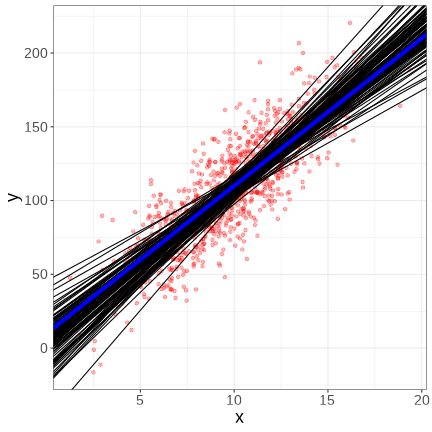
\includegraphics{04_regression2_old_files/figure-beamer/unnamed-chunk-15-1.pdf}
\end{frame}

\begin{frame}[fragile]{Задача}
\protect\hypertarget{ux437ux430ux434ux430ux447ux430-3}{}
Постройте график зависимости стандартизованных остатков от предсказанных
значений

Используйте данные из \texttt{bird\_diag}
\end{frame}

\begin{frame}[fragile]{3. График зависимости стандартизованных остатков
от предсказанных значений}
\protect\hypertarget{ux433ux440ux430ux444ux438ux43a-ux437ux430ux432ux438ux441ux438ux43cux43eux441ux442ux438-ux441ux442ux430ux43dux434ux430ux440ux442ux438ux437ux43eux432ux430ux43dux43dux44bux445-ux43eux441ux442ux430ux442ux43aux43eux432-ux43eux442-ux43fux440ux435ux434ux441ux43aux430ux437ux430ux43dux43dux44bux445-ux437ux43dux430ux447ux435ux43dux438ux439}{}
\begin{Shaded}
\begin{Highlighting}[]
\NormalTok{gg\_resid }\OtherTok{\textless{}{-}} \FunctionTok{ggplot}\NormalTok{(}\AttributeTok{data =}\NormalTok{ bird\_diag, }\FunctionTok{aes}\NormalTok{(}\AttributeTok{x =}\NormalTok{ .fitted, }\AttributeTok{y =}\NormalTok{ .stdresid)) }\SpecialCharTok{+} 
  \FunctionTok{geom\_point}\NormalTok{()}
\NormalTok{gg\_resid}
\end{Highlighting}
\end{Shaded}

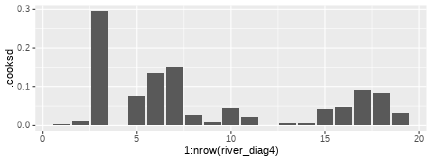
\includegraphics{04_regression2_old_files/figure-beamer/unnamed-chunk-16-1.pdf}

\pause

Разброс остатков не совсем одинаков, но большая часть стандартизованных
остатков в пределах двух стандартных отклонений. Есть отдельные
влиятельные наблюдения, которые нужно проверить. Тренда среди остатков
нет
\end{frame}

\begin{frame}[fragile]{4. Квантильный график стандартизованных остатков}
\protect\hypertarget{ux43aux432ux430ux43dux442ux438ux43bux44cux43dux44bux439-ux433ux440ux430ux444ux438ux43a-ux441ux442ux430ux43dux434ux430ux440ux442ux438ux437ux43eux432ux430ux43dux43dux44bux445-ux43eux441ux442ux430ux442ux43aux43eux432}{}
Используется, чтобы оценить форму распределения. По оси Х --- квантили
теоретического распределения, по оси Y --- квантили остатков модели.

Если точки лежат на одной прямой --- все в порядке.

\begin{Shaded}
\begin{Highlighting}[]
\FunctionTok{library}\NormalTok{(car)}
\FunctionTok{qqPlot}\NormalTok{(bird\_lm, }\AttributeTok{id =} \ConstantTok{FALSE}\NormalTok{) }\CommentTok{\# из пакета car}
\end{Highlighting}
\end{Shaded}

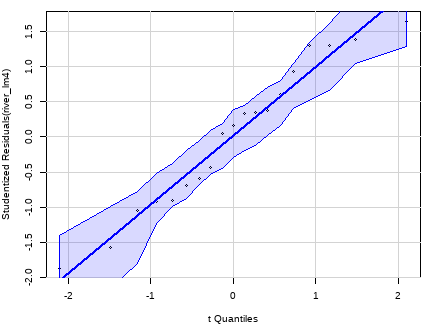
\includegraphics{04_regression2_old_files/figure-beamer/qqplot-1.pdf}
\end{frame}

\begin{frame}{Интерпретируем квантильный график}
\protect\hypertarget{ux438ux43dux442ux435ux440ux43fux440ux435ux442ux438ux440ux443ux435ux43c-ux43aux432ux430ux43dux442ux438ux43bux44cux43dux44bux439-ux433ux440ux430ux444ux438ux43a}{}
Какие выводы можно сделать по квантильному графику?

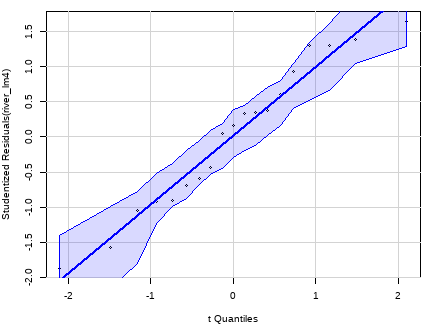
\includegraphics{04_regression2_old_files/figure-beamer/qqplot-1.pdf}
\pause

Отклонений от нормального распределения нет
\end{frame}

\begin{frame}{Внимание!}
\protect\hypertarget{ux432ux43dux438ux43cux430ux43dux438ux435}{}
Только если все условия выполняются, можно приступить к интерпретации
результатов.
\end{frame}

\begin{frame}{Take-home messages}
\protect\hypertarget{take-home-messages}{}
\begin{itemize}
\tightlist
\item
  Для сравнения влияния разных предикторов можно использовать
  бета-коэффициенты
\item
  Условия применимости линейной регрессии должны выполняться, чтобы
  можно было тестировать гипотезы

  \begin{enumerate}
  \tightlist
  \item
    Независимость
  \item
    Линейность
  \item
    Нормальное распределение
  \item
    Гомогенность дисперсий
  \item
    Отсутствие коллинеарности предикторов (для множественной регрессии)
  \end{enumerate}
\end{itemize}
\end{frame}

\begin{frame}{Дополнительные ресурсы}
\protect\hypertarget{ux434ux43eux43fux43eux43bux43dux438ux442ux435ux43bux44cux43dux44bux435-ux440ux435ux441ux443ux440ux441ux44b}{}
\begin{itemize}
\tightlist
\item
  Кабаков Р.И. R в действии. Анализ и визуализация данных на языке R.
  М.: ДМК Пресс, 2014
\item
  Diez, D.M., Barr, C.D. and Çetinkaya-Rundel, M., 2015. OpenIntro
  Statistics. OpenIntro.
\item
  Zuur, A., Ieno, E.N. and Smith, G.M., 2007. Analyzing ecological data.
  Springer Science \& Business Media.
\item
  Quinn G.P., Keough M.J. 2002. Experimental design and data analysis
  for biologists
\item
  Logan M. 2010. Biostatistical Design and Analysis Using R. A Practical
  Guide
\end{itemize}
\end{frame}

\end{document}
